\section{Algoritmo Exacto}

\subsection{Algoritmo}

\indent La idea de este algoritmo es simple. Recorremos la cantidad de colores posibles del grafo g, calculamos su impacto en h y nos quedamos con el máximo.\\
\indent La dificultad del problema radicaba en calcular la cantidad de colores posibles del grafo, algo que a priori puede ser infinito.\\
\indent Consideramos a los colores como números enteros positivos. De aquí se extrae que hay infinitos colores y por lo tanto infinitos coloreos de G válidos.\\
\indent Sin embargo, se pueden hacer algunas consideraciones para acotar considerablemente la cantidad de colores a usar, sin perder generalidad.\\
\indent En primer lugar, intuitivamente se extrae que con $n$ colores es suficiente, donde $n$ es la cantidad de nodos para analizar todos los casos posibles. Entonces consideraremos como colores los primeros $n$ números enteros positivos. Esto es porque en realidad este caso sirve para analizar aquellos donde se tienen $n$ colores distintos, independientemente de que esos $n$ colores no sean los primeros $n$ números positivos (considerando un color como un número).\\
\indent Sin embargo, todavía se puede acotar un poco más las instancias a analizar.\\
\indent Esto tiene que ver con el hecho de que, aunque definamos $n$ colores, uno podría establecer una biyección entre dos conjuntos de colores con los mismos elementos dónde, por ejemplo, en el conjunto 2 se renombra al color 1 del primer conjunto como el color n y viceversa. Esto provocaría, de no tenerse en cuenta, que se estén analizando casos ya analizados. Si además, en vez de renombrar 2 colores los renombrasemos a todos, estaríamos analizando muchísimos casos que, si bien se corresponden a coloreos distintos, son en el fondo, casos equivalentes.\\
\indent Para evitarnos estos análisis de más, determinamos los coloreos de la siguiente manera:\\
\indent Eligimos un nodo cualquiera como el primer nodo para pintar. A ese nodo lo pintamos con el color 1, y por lo que mencionamos anteriormente, de esta manera se estarían analizando también los casos dónde ese nodo tiene otro color entre 2 y n.\\
\indent Ahora se elije otro nodo para pintar en segundo lugar. Para pintarlo tenemos dos posibilidades: o pintarlo del mismo color que el nodo 1 o pintarlo con un color nuevo. Luego, se están generando dos coloreos distintos, y cada uno se sigue generando por separado.\\
\indent La idea es que al pintar el nodo $k$, con $k<=n$, uno podría elegir 2 caminos : o pintarlo de un color ya usado, o pintarlo con un color nuevo.\\
\indent Definamos $max$ como el color de máximo valor utilizado hasta ahora en el coloreo. Luego, existen $max+1$ maneras de continuar ese coloreo, pintando el nodo $k$ de 1,2...$max$ o de un color nuevo, $max+1$.\\
\indent Debe notarse entonces, que por cada paso del coloreo se generan muchos nuevos coloreos más.\\
\indent A medida que se generan los coloreos, generamos otra poda: aquella que determina si al pintar a un nodo de un color se está generando un coloreo válido. En caso de no serlo se deja de analizar ese caso.\\
\indent Luego, de todos los colores posibles válidos se calcula el impacto en H y nos quedamos con aquél que proporciona un máximo impacto.\\

\indent El pseudocódigo del algoritmo es el siguiente:\\   





\begin{algorithm}[H]
\caption{} 
\begin{codebox}
\Procname{$\proc{maximoImpactoExacto}(Grafo$ g$, Grafo$ h$)$}

\li vector$<$unsigned int$>$ $res(n+1)$
\li int $res[0] \gets 0$
\li vector$<$unsigned int$>$ $coloreo(n,0)$
\li $coloreo[0] \gets 1$
\li $colorear(1,g,h,coloreo,res)$
\li	return $res$
\End
\end{codebox}
\end{algorithm}


\begin{algorithm}[H]
\caption{} 
\begin{codebox}
\Procname{$\proc{colorear}(unsigned$ $int$ nodo, $Grafo$ g$, Grafo$ h$, $vector$<$unsigned int$>$ coloreo$, $vector$<$unsigned int$>$ solucion$)$}

\li \If (nodo $>$ n) \Do
\li 	$int$ temp $\gets$ impacto(h, coloreo)
\li		\If $temp > solucion[0]$ \Do
\li			$solucion[0] \gets temp$
\li			\For i desde 0 hasta n \Do
\li				$solucion[i+1]=coloreo[i]$
			\End
		\End
	\End
\li \Else \Do
\li		$int$ maxColor $\gets $ maximo color usado hasta el momento 	
\li		\For c desde 1 hasta maxColor \Do
\li			\If es legal pintar el nodo $nodo$ del color c \Do
\li				vector$<$unsigned int$>$ nuevoColoreo(coloreo)
\li             $nuevoColoreo[nodo] \gets c$
\li             $colorear(nodo+1,g,h,nuevoColoreo,solucion)$
             \End
         \End
\End
\end{codebox}
\end{algorithm}


\subsection{Análisis de complejidad}

\indent Al momento de hacer este análisis de complejidad se tuvieron en cuenta algunas consideraciones.\\
\indent En primer lugar, llamaremos $m$ al máximo entre la cantidad de aristas del grafo G y del grafo H  y $n$ a la cantidad de nodos de dichos grafos.\\
\indent En segundo lugar, en el análisis de complejidad de la función $colorear$ se definirá $k$ como la cantidad de nodos que quedan por pintar hasta ese paso de la recursión, en contraste con la implementación donde la recursión es , por así decirlo $hacia arriba$, significando esto que se inicia desde el primer nodo y se va hacia el último.\\

\indent Analicemos primero la función $colorear$. Como mencionamos anteriormente, consideraremos la recursión en la cantidad de nodos que quedan por colorear.

\indent El caso base será cuando no hayan más nodos por pintar. En dicho caso, el algoritmo simplemente calcula el impacto de dicho coloreo en el grafo H y en caso de ser el de máximo impacto hasta el momento se reemplaza la solución anterior por la nueva. Esto cuesta O(n+m), que es lo que cuesta calcular el impacto en H.\\
\indent Para el caso en el que la cantidad de nodos a pintar sea distinta de cero, el algoritmo calcula los posibles colores con los que pintar el nodo. Esto lo hace buscando cuál es el máximo color usado hasta el momento. El nuevo nodo podrá ser pintado de los colores usados anteriormente o del máximo color usado hasta el momento + 1, es decir pintándolo de un nuevo color. Esto se calcula en tiempo O(n).Luego se llamará a la función recursivamente una cantidad de veces igual al máximo color a utilizar. Ese valor se puede acotar para todos los casos por n-k+1.\\
\indent Además se chequea que agregar ese color genere un coloreo válido, y eso cuesta O(cantidad de vecinos del nodo), que lo podemos acotar por la cantidad de aristas de G, es decir O(m). Luego se hace la llamada recursiva para la instancia inmeditamente menor.\\
\indent Pasando en limpio, en el paso $k$ el algoritmo cuesta (n-k+1)*(n+m + T(k-1)).\\
\indent Es decir:\\

\indent T(0)=n+m\\
\indent T(k)=(n-k+1)*[(n+m)+ T(k-1)]\\

donde $k$ es la cantidad de nodos que quedan por pintar.\\


\indent Veamos entonces cuánto cuesta pintar todos los nodos.\\
\indent Basado en la definición que dimos antes, si tenemos que pintar todos los nodos, estamos en el caso T(n).\\

\indent T(n)=(n-n+1)*(n+m + T(n-1))\\

\indent Desarrollemos T(n):\\


\begin{centering}
T(n)=(n-n+1)*(n+m + T(n-1))=\\
= n+m + [2*(n+m) + 2*T(n-2)]=\\
=(n+m)+2*(n+m) + 2*[3*(n+m)+ 3* T(n-3)]=\\
=(n+m)+2*(n+m)+ 2*3*(n+m) + 2*3 T(n-3)=\\
=(n+m)+2*(n+m)+ 2*3*(n+m) + 2*3*[4*(n+m)+4*T(n-4)]=\\
=(n+m)+2*(n+m)+2*3*(n+m)+2*3*4*(n+m)+ 2*3*4*T(n-4)=\\
=...=\\
=[ $\sum_{i=1}^{n} i! * (n+m) $] + n! * T(0)= \\
=[ $\sum_{i=1}^{n} i! * (n+m) $] + n! * (n+m)\\
\end{centering}


\indent Es decir que T(n)= [ $\sum_{i=1}^{n} i! * (n+m) $] + n! * (n+m)\\

\indent Conjeturamos entonces que T(n) es O($\sum_{i=1}^{n} i! * (n+m) $).\\

\indent Veámoslo por inducción en la cantidad de nodos por pintar:\\

\indent Queremos ver que existe un $d$ real positivo y $n_{0}$ natural positivo tales que para todo $n\geq n_{0}$ vale que $T(n) \leq d * [\sum_{i=1}^{n} i! * (n+m)] $.

\indent Caso base: n=1 \\

\begin{center}
T(1)= $\sum_{i=1}^{1} i! * (1+m)  1! * (1+m) $ = 2*1!*(1+m) =\\
=2*(1+m) $\leq$ 2*  $\sum_{i=1}^{1} i! * (1+m)$ \\
\end{center}

\indent Es decir que con un $d=2$ nos alcanza.\\


\indent Paso inductivo: Suponiendo que vale que $T(n-1) \leq d * [\sum_{i=1}^{n-1} i! * (n-1+m)] $ quiero ver que vale $T(n) \leq d * [\sum_{i=1}^{n} i! * (n+m)] $ \\


\begin{center}
T(n)=(n-n+1)*(n+m + T(n-1))=\\

= (n+m) + T(n-1)$\leq$\\

$\leq$ por hipótesis inductiva $\leq$\\

$\leq n+m + d * [\sum_{i=1}^{n-1} i! * (n-1+m)] \leq $\\

$\leq n+m + d * [\sum_{i=1}^{n-1} i! * (n+m)] \leq$ \\

$\leq (n+m) *[ (d* \sum_{i=1}^{n-1} i!) + 1] \leq$ \\

$\leq (n+m) *[ (d* \sum_{i=1}^{n-1} i!) + n!] \leq$ \\

$\leq (n+m) *[ (d* \sum_{i=1}^{n} i!)] \leq$\\

$\leq  d* \sum_{i=1}^{n} i!*(n+m)$\\

\end{center}

\indent que es lo que queríamos ver.\\

\indent Luego, colorear cuesta O($\sum_{i=1}^{n} i! * (n+m) $).\\

\indent maximoImpactoExacto cuesta entonces O(n+1 + n + 1 + $\sum_{i=1}^{n} i! * (n+m) $) que es O($\sum_{i=1}^{n} i! * (n+m) $).\\

\subsection{Experimentación y Resultados}
\quad Trabajamos con los siguientes 3 casos: grafos al azar, grafos densos, G y H complementos.

\quad Se midieron los tiempos en corridas de  5 a 100 nodos con 100 repeticiones para cada cantidad de nodos.

\subsubsection{Grafos al azar}

\begin{figure}[H]
	\centering
	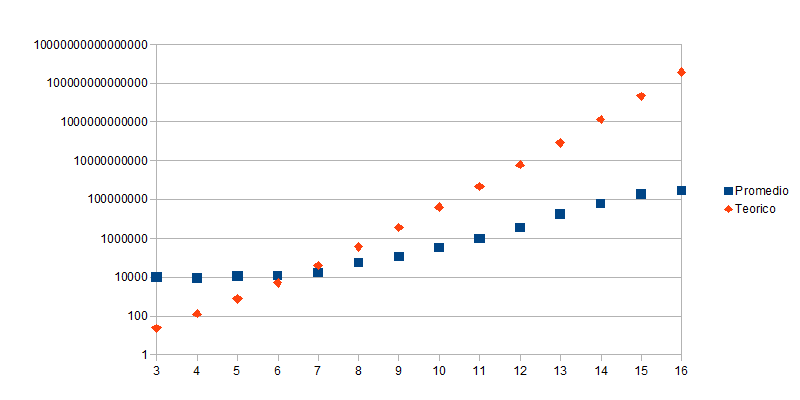
\includegraphics[scale=0.8]{exacto-tiempos-Azar.png}
\caption{Costos}
\end{figure}

\subsubsection{Grafos densos}

\begin{figure}[H]
	\centering
	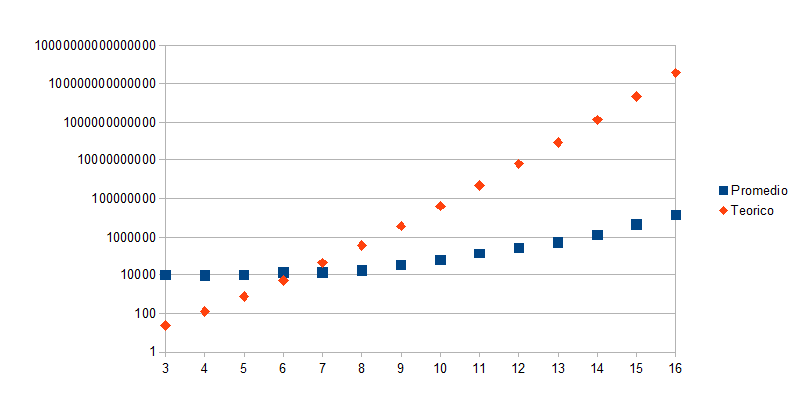
\includegraphics[scale=0.8]{exacto-tiempos-G-y-H-densos.png}
\caption{Costos}
\end{figure}

\subsubsection{G y H complementos}

\begin{figure}[H]
	\centering
	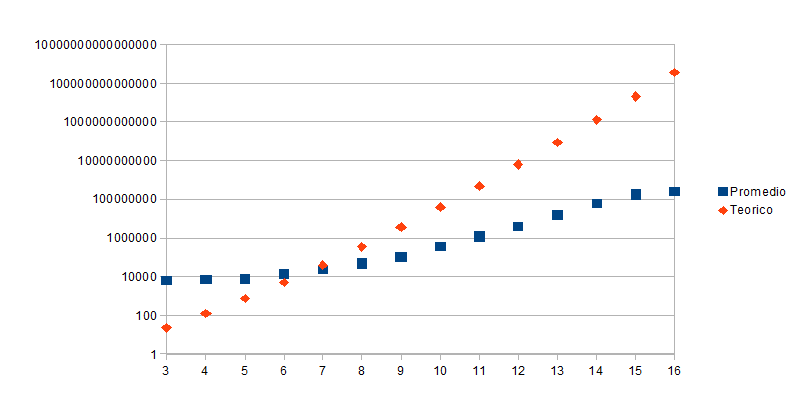
\includegraphics[scale=0.8]{exacto-tiempos-H-complemento.png}
\caption{Costos}
\end{figure}